\chapter{Development of Recommendation
System}
\section*{Introduction}
This chapter presents the architectural design, implementation methodology, and empirical evaluation of the hybrid recommendation system
developed for the VitamiNurse mobile application. The system employs
a multi-modal architecture that integrates collaborative filtering, contentbased filtering, and real-time behavioral analytics to deliver personalized
nutritional recommendations aligned with users’ health profiles, dietary
restrictions, and preferences.
The chapter begins with an analysis of vector databases as foundational
infrastructure for semantic retrieval, including a detailed discussion of approximate nearest neighbor (ANN) search and the Hierarchical Navigable
Small World (HNSW) algorithm. Subsequent sections detail the system’s
hybrid architecture, algorithmic components, embedding strategies, and
deployment pipeline.

\section{Vector Databases and Semantic Retrieval}
Vector databases serve as the backbone of modern content-based recommendation systems by enabling efficient similarity search in highdimensional embedding spaces.
In VitamiNurse, they facilitate the semantic matching of user health
profiles with nutritional products based on dietary needs, allergies, and
wellness goals.
\subsection{Fundamentals of Vector Databases}
Vector databases store and index dense numerical representations (embeddings) of data objects, allowing retrieval based on semantic similarity
rather than exact keyword matches [14]. Each item is mapped to a point
in a continuous vector space, where proximity reflects conceptual relatedness. Similarity is typically measured using cosine distance or Euclidean
norms, enabling applications such as semantic search, recommendation,
and clustering.

\begin{figure}[H]
\centering
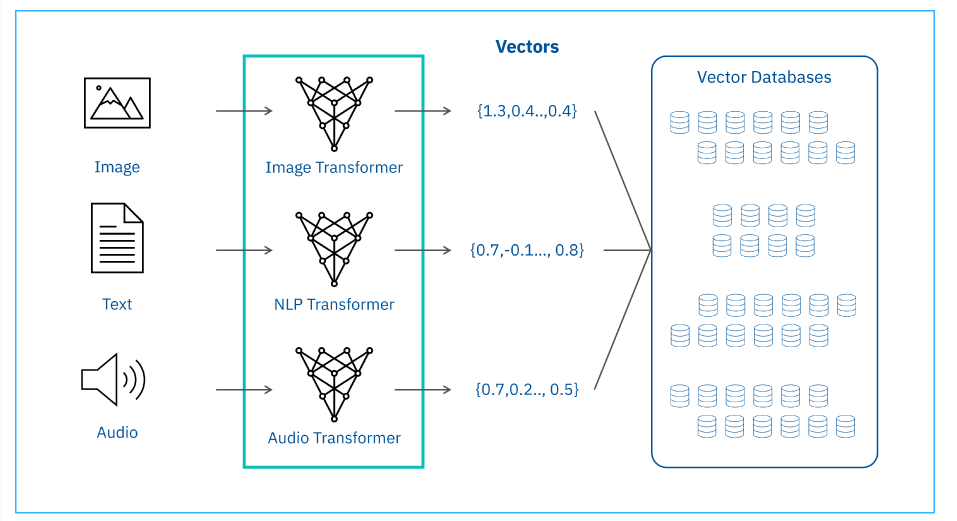
\includegraphics[scale=0.45]{images/vectorDB.png}
\caption{Embedding representation in a vector database}
\label{fig:vectorDB}
\end{figure}

\subsection{Approximate Nearest Neighbor Search}
Based on comparing a query vector against all stored vectors, exact
similarity search becomes computationally prohibitive as dataset size
grows particularly in high-dimensional spaces due to the “curse of dimensionality” [15].
Approximate Nearest Neighbor (ANN) algorithms address this limitation
by sacrificing marginal accuracy for substantial gains in speed and memory
efficiency. These methods construct specialized index structures (e.g.,
trees, hash tables, or graphs) that enable sublinear-time retrieval of
near-optimal neighbors.
\subsection{HNSW Algorithm}
Among ANN techniques, the Hierarchical Navigable Small World (HNSW)
algorithm has emerged as a state-of-the-art solution for large-scale similarity search [16]. HNSW organizes vectors into a multi-layer graph: upper
layers contain sparse, long-range connections for rapid coarse navigation,
while lower layers provide dense, local links for fine-grained refinement.
Search begins at the top layer and descends iteratively, achieving logarithmic time complexity with high recall. This balance of speed and
accuracy makes HNSW ideal for real-time recommendation systems.
\subsection{Selection of ChromaDB}
ChromaDB was selected as the vector database for VitamiNurse due to
its native support for HNSW indexing and native support for HNSW
indexing under an open-source license [17]. A critical feature is its ability
to update the vector index dynamically without full retraining, which is
essential for the system’s daily synchronization of product metadata from
external retailers. Additionally, ChromaDB supports metadata filtering
alongside vector search, allowing post-retrieval enforcement of health
constraints such as excluding gluten-containing products for celiac users.

\begin{figure}[H]
    \centering
    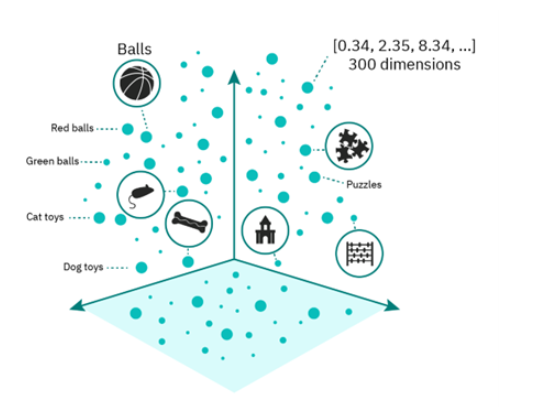
\includegraphics[scale=0.66]{images/chroma_space.png}
    \caption{Vector search mechanism in ChromaDB using HNSW}
    \label{fig:vector_search}
\end{figure}

\subsection{Vector Search Versus Traditional Keyword Search}
Traditional search relies on discrete tokens and exact matching, limiting
its ability to generalize across semantically related terms. In contrast,
vector search retrieves items based on embedding proximity. For example,
a query for “dark chocolate” may return “organic cacao snacks” if their
embeddings are close, even in the absence of shared keywords. This
capability is essential for delivering nutritionally appropriate alternatives
that align with user health objectives.

\subsection{Embedding Generation}
Dense vector representations are produced using transformer-based sentence encoders. These models map textual descriptions of products and
user profiles into fixed-dimensional spaces where semantic relationships
are preserved geometrically. Efficient indexing and retrieval of these
embeddings are enabled by ANN algorithms such as HNSW, ensuring
scalability without compromising relevance.

\section{System Architecture}
VitamiNurse employs a \textbf{modular hybrid architecture}, separating
collaborative and content-based filtering into specialized components:

\item \textbf{CLightFM (Pure Collaborative):} I Captures long-term user preferences via matrix factorization, trained only on interaction data to avoid metadata-induced noise.
\item \textbf{ChromaDB (Content-Based):}  Handles real-time product similarity using HNSW, enabling rapid updates without model retraining.
\subsection{Hybrid Architecture Design}
VitamiNurse implements a hybrid recommendation system that combines
offline collaborative filtering (CF) with real-time, nutrition-aware contentbased filtering (CBF). The collaborative component uses LightFM, trained
nightly at 00:00 on user interaction data (views, likes, dislikes) to capture
long-term preferences without metadata bias. In parallel, a contentbased pathway leverages ChromaDB with HNSW indexing to perform
low-latency similarity searches over product embeddings generated by
the all-MiniLM-L6-v2 model.

When a user scans a product, the system retrieves semantically similar
items and re-ranks them according to the nutrition profile of the user.
This profile is continuously updated in real-time by its interactions with
the Nutrition AI Assistant.

Final recommendations are produced via a weighted ensemble (60\%
content-based, 40\% collaborative), prioritizing immediate nutritional
relevance while retaining historical preference signals. The architecture is
organized into four layers—data ingestion, embedding generation, hybrid
recommendation, and API serving—enabling scalable, responsive, and
health-conscious personalization.

\begin{figure}[H]
\centering
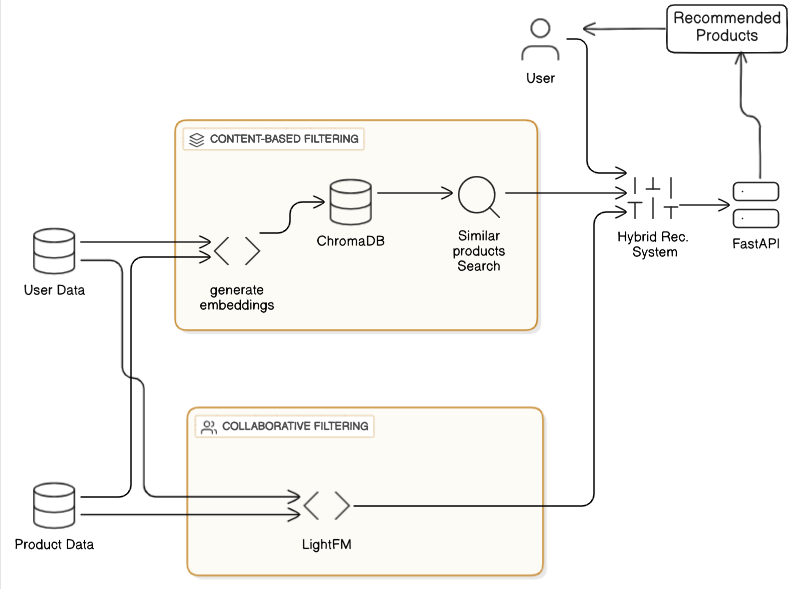
\includegraphics[scale=0.55]{images/RS_Arch.png}
\caption{Overall architecture of the recommendation system}
\label{fig:Recommendation_Sequence_Diagram}
\end{figure}

\subsection{Hybrid System with Decoupled Components}
Although the LightFM framework supports two principal modes : \textbf{pure
collaborative filtering} and \textbf{hybrid filtering}, we chose to employ only
the pure collaborative model for VitamiNurse’s recommendation system.
The system integrates collaborative filtering (CF) and content-based
filtering (CBF) through a weighted ensemble approach. These approaches
are combined in a hybrid recommender, which assigns weighted scores
(60\% content-based powered by ChromaDB, 40\% collaborative with
LightFM) to rank recommendations. This decision was made after
extensive evaluation and careful alignment with the platform’s realtime infrastructure requirements. The selected approach offers greater
scalability and modularity, particularly given the dynamic nature of our
product catalog and metadata. The following subsections outline the key
architectural and empirical factors that guided this choice.
\\
\textbf{Why Not LightFM Hybrid?}
\\
While hybrid models are often assumed to enhance performance by
incorporating additional features, we avoided LightFM’s hybrid mode for
the following reasons:

\paragraph{1) Real-time Product Updates and Scalability Requirements}

VitamiNurse’s product database synchronizes daily with external retail inventories, meaning metadata (e.g., categories, availability) can change frequently. A hybrid LightFM model would require retraining whenever item features update, introducing latency and scalability challenges. In contrast, our content-based filtering module (powered by ChromaDB with HNSW-based approximate nearest neighbor search) dynamically adapts to metadata changes without retraining, making it better suited for real-time updates [18].

ChromaDB’s vector infrastructure is optimized for large-scale similarity
search, supporting millions of product embeddings with efficient retrieval.
This eliminates the need to encode metadata directly into LightFM, as
the content-based component handles this asynchronously and with lower computational overhead.
\paragraph{2) Benchmark Evidence

Pure LightFM Outperforms Hybrid LightFM}
Empirical studies consistently demonstrate that LightFM’s pure collaborative
model achieves superior performance compared to its hybrid counterpart:

\begin{itemize}
\item \textbf{MovieLens 100k Benchmark:} [19] evaluated LightFM on the
MovieLens dataset, showing that the pure model outperformed the
hybrid variant in precision@K and recall@K across cutoffs (K=5, 10,
20). The hybrid model not only underperformed but also failed to
surpass simpler baselines like ItemKNN in some metrics as illustrated
in Figure 4.4.
\item \textbf{Feature Noise:} The inclusion of item features degraded performance, likely due to redundant or poorly weighted metadata. [19]
found that the hybrid model’s precision\@5 was worse than graphbased baselines like P3\α and RP3\β.
\item \textbf{Community Reports:} GitHub issues and user reports corroborate
these findings, with cases where shuffled or irrelevant item features
further reduced model accuracy [20].
\end{itemize}

\paragraph{3) Computational Efficiency}

Pure collaborative filtering requires fewer
computational resources during training and inference. Benchmarks on
the Movielens 20M dataset show that LightFM’s inference speed scales
linearly with latent factor dimensionality, but hybrid models introduce
additional overhead from feature processing.

This decoupling aligns with industry best practices, where hybrid \textit{systems} (not hybrid \textit{models}) often deliver more robust performance. This
architecture ensures scalability while maintaining interpretability and
efficiency.
\subsection{Dynamic Data Update and Sync Architecture}
The VitamiNurse system operates through a robust, modular data
pipeline designed for real-time responsiveness and adaptability to both
user behavior and product catalog changes:
\begin{enumerate}
\item \textbf{ Real-time Interaction Tracking:} 

User activities, such as viewing, liking, and disliking products, are continuously monitored and
recorded. These interactions directly inform the recommendation
engine, ensuring up-to-date and personalized suggestions.
\item \textbf{Dynamic Profile Synchronization:} 

Upon any profile change
(e.g., allergy updates, changed health conditions, pregnancy status),
the system triggers immediate re-embedding of the user’s profile
vector within ChromaDB. This ensures atomic, consistent updates
that instantly reflect in recommendations, without disrupting the
user’s session.
\item \textbf{ Automated Product Ingestion and Embedding:} 

The product
catalog is synchronized daily with partner retailers. New or modified
products are automatically detected, vectorized through semantic
embedding, and integrated into the recommendation graph using a
CDC (Change Data Capture) pipeline.

\item \textbf{Daily Model Retraining:}

To adapt to evolving user preferences
and product changes, the LightFM recommendation model is retrained every 24 hours (scheduled at 00:00 UTC). This ensures
continuous learning and optimal recommendation quality.
\end{enumerate}

\section{Content-based filtering}
The content-based (CB) recommendation module in VitamiNurse is
designed to provide personalized nutritional product suggestions by leveraging semantic similarity between user profiles and product characteristics.
This is achieved through dense vector embeddings stored in ChromaDB
and computed using a lightweight sentence-transformer model.

\subsection{Embedding Model Evaluation}


\begin{table}[h!]
\centering
\resizebox{0.9\textwidth}{!}{%
\begin{tabular}{@{}lccccc@{}}
\toprule
\textbf{Model Name} & \textbf{Sent. Emb.} & \textbf{Sem. Search} & \textbf{Avg. Perf.} & \textbf{Speed} & \textbf{Size} \\
\midrule
\textbf{all-mpnet-base-v2} & \textbf{69.57} & \textbf{57.02} & \textbf{63.30} & \textbf{2800} & 420 MB \\
multi-qa-mpnet-base-dot-v1 & 66.76 & 57.60 & 62.18 & 2800 & 420 MB \\
all-distilroberta-v1 & 68.73 & 50.94 & 59.84 & 4000 & 290 MB \\
all-MiniLM-L12-v2 & 68.70 & 50.82 & 59.76 & 7500 & 120 MB \\
multi-qa-distilbert-cos-v1 & 65.98 & 52.83 & 59.41 & 4000 & 250 MB \\
\textbf{all-MiniLM-L6-v2} & \textbf{68.06} & \textbf{49.54} & \textbf{58.80} & \textbf{14200} & 80 MB \\
multi-qa-MiniLM-L6-cos-v1 & 64.33 & 51.83 & 58.08 & 14200 & 80 MB \\
paraphrase-multilingual-mpnet-base-v2 & 65.83 & 41.68 & 53.75 & 2500 & 970 MB \\
paraphrase-albert-small-v2 & 64.46 & 40.04 & 52.25 & 5000 & 43 MB \\
paraphrase-multilingual-MiniLM-L12-v2 & 64.25 & 39.19 & 51.72 & 7500 & 420 MB \\
paraphrase-MiniLM-L3-v2 & 62.29 & 39.19 & 50.74 & 19000 & 61 MB \\
distiluse-base-multilingual-cased-v1 & 61.30 & 29.87 & 45.59 & 4000 & 480 MB \\
distiluse-base-multilingual-cased-v2 & 60.18 & 27.35 & 43.77 & 4000 & 480 MB \\
\bottomrule
\end{tabular}
}
\caption{Performance comparison of SentenceTransformer models. Speed is measured as average sentences processed per second.}
\label{tab:models}
\end{table}
Speed is measured as average
sentences processed per second.
\\
 The \textit{SentenceTransformers} library offers a range of models evaluated for
their performance in generating sentence embeddings and conducting
semantic search, based on two key criteria: the quality of cross-sentence
representations across 14 datasets and the effectiveness in semantic search
tasks on 6 datasets.
The \textbf{all-*} models, trained on an extensive corpus of over one billion text
pairs, are designed as general-purpose models, with \textit{all-mpnet-base-v2} delivering the highest overall quality and \textit{all-MiniLM-L6-v2} providing comparable quality at approximately five times the speed, making it an
efficient choice for various applications [21].


\subsection{Embedding Model Selection}
The system employs the all-MiniLM-L6-v2 model for generating embeddings, which offers several advantages over alternatives. By being
fine-tuned on over 1 billion text pairs, the all-MiniLM-L6-v2 excels in
semantic similarity tasks. Despite its smaller size, it achieves 93\% the
accuracy of larger models such as BERT-base models.
This sentence transformer model is an excellent choice for VitamiNurse
recommendation system, as it produces 384-dimensional embeddings that
effectively capture subtle relationships within the data. [22] Furthermore,
its compact architecture, with only 33.4 million parameters, enables
efficient CPU-only inference, and multilingual support enables global
applicability. The model’s balance of speed, accuracy, and resource
efficiency makes it ideal for real-time recommendation scenarios in the
VitamiNurse application.
\subsection{CB Recommendation Process}

\paragraph{Query Construction}
\\
The CB system operates based on two possible inputs: the \textbf{user identifier}
and an optional \textbf{scanned product identifier} (EAN code). When a
user scans a product, the system retrieves metadata associated with that
item such as product name, brand, categories, and nutrition information.
Simultaneously, it extracts the user’s profile information, which includes
dietary preferences, pregnancy status, and medical conditions like diabetes
or hypertension.\\
These two sources of information are merged to create a descriptive
query that captures both the scanned product’s features and the user’s
health-related needs.
\paragraph{Search and Recommendation}

The query is then embedded into a vector using the selected embedding
model and used to perform a semantic search in the product database.
The search returns a list of nutritionally and semantically similar products.
In cases where no product is scanned, the recommendation relies entirely
on the user’s profile to infer their preferences and health requirements.
Based on this information, it generates a personalized query, which is
then used to display tailored recommendations on the home page.

\paragraph{Recommendation Score}

Each recommended product is assigned a relevance score based on semantic proximity. This score is further refined by applying domain specific
nutritional rules by boosting products with better Nutri-Scores. The
system also applies post-filtering to strictly enforce compatibility with
medical conditions or dietary restrictions. For instance, a user with celiac
disease will never be recommended a product that contains gluten, even
if it is semantically similar.
\paragraph{CB Recommendation Workflow}

The content based recommendation workflow follows a structured process
in order to offer a personalized and health-aware user experience, as
illustrated in the following diagram. It begins by metadata gathering
and query construction. Queries are embedded into vectors using the allMiniLM-L6-v2 model for semantic search against the product database.
The system then selects and returns recommendations aligned with user
preferences and nutritional needs.\\
This design ensures that the products delivered by the content based
recommendation system are not only contextually relevant but also
aligned with the unique nutritional profile of each user of VitamiNurse
app.
\section{Collaborative Filtering}
Collaborative filtering in \textit{VitamiNurse} leverages the \textbf{LightFM model},
which combines matrix factorization and metadata-aware learning.
\subsection{Overview}
Collaborative filtering (CF) is a widely used recommender system technique that predicts user preferences by leveraging the collective behavior
of similar users or items. As defined by IBM, CF operates on the principle
that users with shared interests in the past will likely agree in the future, making recommendations based on patterns identified in user-item
interaction matrices [23].

\begin{figure}[H]
\centering
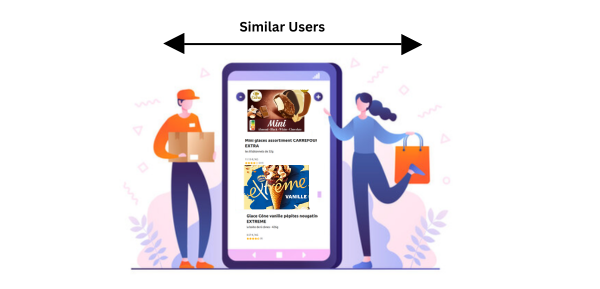
\includegraphics[scale=0.85]{images/collaborative_filtering.png}
\caption{Collaborative filtering logic}
\label{fig:cf_workflow}
\end{figure}

\subsection{LightFM’s Collaborative Filtering Approach
}
LightFM implements a hybrid matrix factorization model rather than
traditional memory-based (neighborhood) collaborative filtering. Unlike
user/item-neighborhood methods that rely on cosine similarity or Pearson
correlation [23], LightFM learns latent embeddings using Weighted Matrix
Factorization (WMF) or Bayesian Personalized Ranking (BPR) loss. This
approach is scalable and well-suited for sparse datasets, making it ideal
for recommendation systems like VitamiNurse.

\subsection{ Creation of the Interaction Matrix}
VitamiNurse incorporates multiple types of user feedback, each assigned
specific weights to reflect varying degrees of preference:

Table 4.2: Interaction types and corresponding weight values
\\
\\
manque le tableau


\\

\subsection{Loss Functions in LightFM}
The LightFM library supports multiple loss functions tailored to different
recommendation scenarios:
\begin{itemize}
\item \textbf{WARP} (Weighted Approximate-Rank Pairwise): Optimized for
ranking tasks with implicit feedback (clicks). It focuses on positive signals and is effective for top-N recommendations but does not
handle negative feedback well.
\item \textbf{BPR} (Bayesian Personalized Ranking): Designed for personalized
item ranking through pairwise comparisons. It ranks preferred items
higher than less preferred or irrelevant ones, accommodating nuanced
feedback.
\item \textbf{Logistic}: Used for probabilistic modeling, typically with explicit
feedback (ratings)
\end{itemize}

\subsection{ Selection of Loss Function}
The selection of an appropriate loss function is critical in recommendation
systems, as it determines how user-item interactions are modeled during
the training process. Collaborative filtering leverages implicit feedback
(likes, views, dislikes) weighted as shown in Table 4.2 to inform this
process.

Our collaborative module cannot use WARP loss because it fails to model
explicit dislikes (-1.0). Instead, \textbf{Bayesian Personalized Ranking}
(BPR) was chosen because it optimizes pairwise comparisons, explicitly
ranking liked items higher than visited or disliked ones while leveraging
both positive and negative signals. This approach better aligns with
VitamiNurse’s goal of learning from complex user interactions while
maintaining scalability on sparse datasets.

\section{Benchmarking the Recommendation System:
Exact vs. ANN (HNSW) Search}

To ensure both scalability and precision, we benchmarked two vector
search modes available in ChromaDB: the default exact search and the
HNSW-enabled Approximate Nearest Neighbor (ANN) search.
\subsection{Theoretical Comparison}
Exact search is ChromaDB’s default method . It performs exhaustive
comparisons between the query vector and all stored vectors using cosine
similarity, ensuring maximum precision. However, this method can
become computationally expensive as the dataset grows.
As we have seen, HNSW search is an approximate nearest neighbor
(ANN) technique that is frequently adopted in large-scale recommender
systems. It constructs a navigable graph index that accelerates retrieval.
Although it introduces a slight drop in precision, it significantly enhances
speed and scalability.
The following table summarizes the key differences between the two
modes:
\\

Table 4.3: Key Differences: Default vs. HNSW Search
\\
\\

\subsection{Experimental Results and Scalability Implications}
We benchmarked 20,000 recommendation requests using ChromaDB with
23,000 products indexed. Both modes—Exact (port 8000) and HNSW
(port 8001) returned valid top-10 results for each request with a 100\%
success rate.

\\
Table 4.4: Benchmark Results for Recommendation Modes

\\
Results demonstrate that \textbf{HNSW} significantly outperforms exact search
in terms of speed (from 187.4ms to 178.08ms), even with only 23,000
products. As VitamiNurse scales to hundreds of thousands or even
millions of products across Europe and the US, the cost of exact search
will become increasingly prohibitive.
HNSW, by contrast, offers scalable performance with near-equivalent
accuracy, making it the preferred choice for large-scale deployments in
real-time production environments.
Results demonstrate that \textbf{HNSW} significantly outperforms \textbf{exact
search} on speed while maintaining high relevance in practical use cases.
It is now the preferred mode for large-scale deployments in VitamiNurse.

\section{ Deployment}
\subsection{FastAPI Deployment}
To facilitate real-time access to personalized nutritional recommendations
within the \textit{VitamiNurse} mobile application, the recommendation engine
is exposed through a RESTful API developed using a private \textbf{FastAPI}
service. We chose FastAPI for its performance, asynchronous capabilities,
and automatic data validation using Pydantic.

Our API provides a single endpoint, \/recommend, which receives structured input from the app (user ID, scanned EAN,limit, recommendation\_type) and returns tailored food item suggestions in JSON format.

\subsection{ Multi-Modal Recommendation Deployment}
The API supports three recommendation modes selectable via a recommendation type parameter:
\begin{enumerate}
\item Collaborative filtering
\item Content-based filtering
\item  Hybrid approach
\end{enumerate}
This internal service ensures fast, reliable, and scalable communication
between the app and the recommendation system. Although fully documented through FastAPI’s auto-generated Swagger UI, the API will be
accessed exclusively by the mobile app and the development team for
testing.

\begin{figure}[H]
\centering
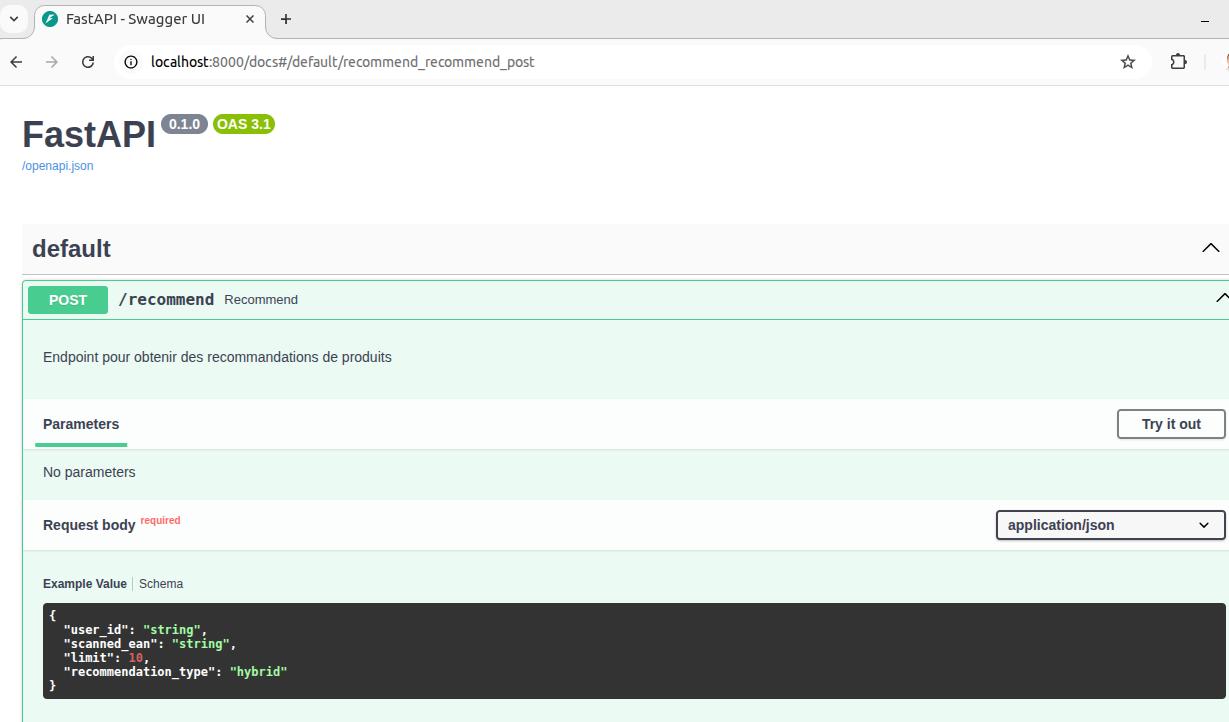
\includegraphics[scale=0.35]{images/swaggerFastAPI.png}
\caption{Swagger UI for the internal Recommendation API}
\label{fig:swagger_UI}
\end{figure}













\paragraph{2. Empirical Performance}
Benchmarking on MovieLens 100k \cite{shu2023lightfm} shows:
\item Pure LightFM outperforms hybrid LightFM in precision@K and recall@K.
    \item Item features often introduce noise, degrading performance.
    \item Hybrid LightFM underperforms simpler baselines like ItemKNN and RP3$\beta$.

\begin{figure}[H]
    \centering
    \begin{minipage}{0.48\textwidth}
        \centering
        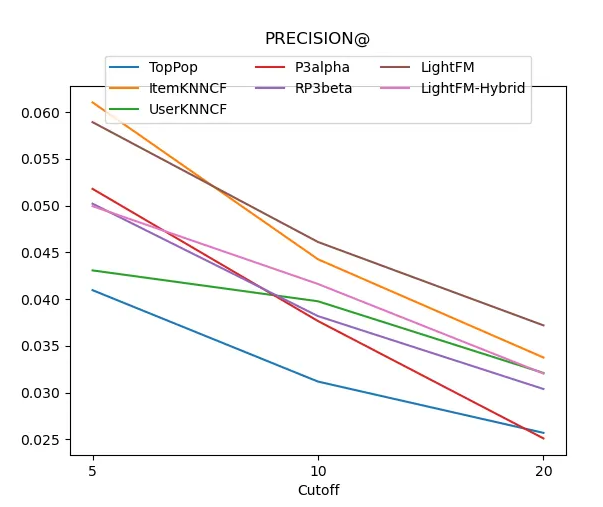
\includegraphics[width=\linewidth]{images/precision_plot.png}
        \caption{Precision@K comparison}
        \label{fig:precision}
    \end{minipage}\hfill
    \begin{minipage}{0.48\textwidth}
        \centering
        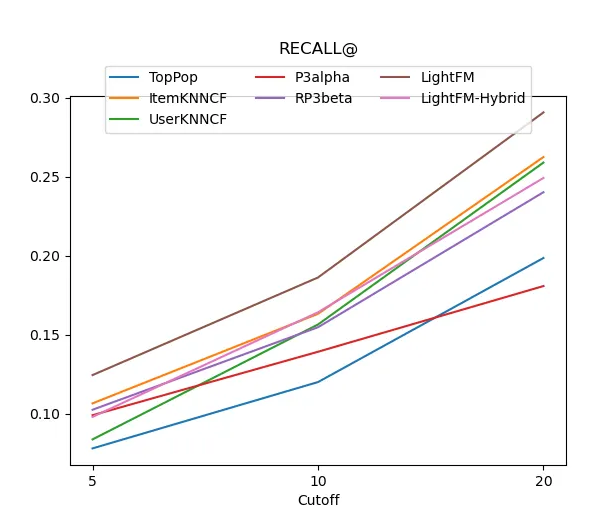
\includegraphics[width=\linewidth]{images/recall_plot.png}
        \caption{Recall@K comparison}
        \label{fig:recall}
    \end{minipage}
\end{figure}

\paragraph{3. Computational Efficiency}
Pure CF reduces training/inference overhead, enabling faster daily retraining and lower operational costs.

This decoupled approach aligns with industry best practices: **hybrid systems** (not hybrid models) offer greater flexibility and maintainability.

\subsection{Dynamic Data Pipeline}
The system supports continuous adaptation through:
\begin{enumerate}
    \item \textbf{Real-time interaction logging}
    \item \textbf{Profile-triggered re-embedding} (e.g., allergy updates)
    \item \textbf{CDC-based product ingestion} (Change Data Capture from retailers)
    \item \textbf{Daily LightFM retraining} (scheduled at 00:00 UTC)
\end{enumerate}

\section{Content-Based Filtering Module}
\subsection{Semantic Personalization via Embeddings}
The CBF module generates recommendations by computing semantic similarity between:
\item User profile (dietary preferences, health conditions)
    \item Product metadata (name, category, nutrition facts, allergens)

\begin{figure}[H]
\centering
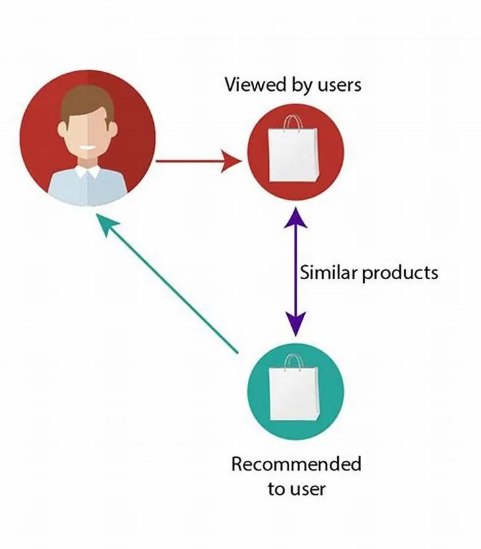
\includegraphics[scale=0.35]{images/cb_filtering_logic.png}
\caption{Logic of content-based filtering in VitamiNurse}
\label{fig:CB_filtering_logic}
\end{figure}

\subsection{Embedding Model Selection}
We evaluated multiple SentenceTransformer models (Table~\ref{tab:models}). \texttt{all-MiniLM-L6-v2} was selected for its optimal trade-off:

\begin{table}[H]
\centering
\caption{Performance comparison of SentenceTransformer models}
\label{tab:models}
\resizebox{0.9\textwidth}{!}{%
\begin{tabular}{@{}lccccc@{}}
\toprule
\textbf{Model} & \textbf{Sent. Emb.} & \textbf{Sem. Search} & \textbf{Avg. Perf.} & \textbf{Speed (sent/s)} & \textbf{Size} \\
\midrule
all-mpnet-base-v2 & 69.57 & 57.02 & 63.30 & 2800 & 420 MB \\
\textbf{all-MiniLM-L6-v2} & \textbf{68.06} & \textbf{49.54} & \textbf{58.80} & \textbf{14200} & \textbf{80 MB} \\
\bottomrule
\end{tabular}%
}
\end{table}

It achieves 93\% of BERT-base accuracy with 5× faster inference and minimal memory footprint—ideal for mobile backend deployment.

\subsection{Data Ingestion into ChromaDB}
Product metadata is embedded using \texttt{all-MiniLM-L6-v2} and loaded into ChromaDB with HNSW indexing. The compact 384-dimensional vectors enable efficient CPU-based inference and multilingual support.

\begin{figure}[H]
\centering
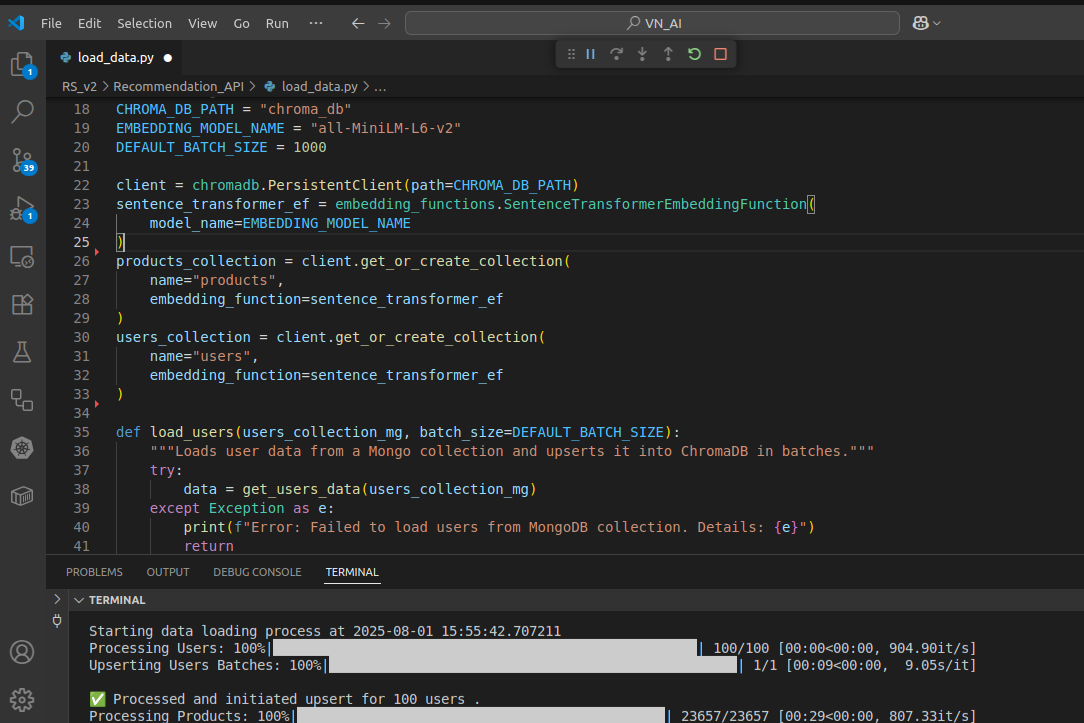
\includegraphics[scale=0.39]{images/load_data__0.png}
\caption{Data loading pipeline into ChromaDB}
\label{fig:load_data_chroma}
\end{figure}

\subsection{Recommendation Workflow}
\subsubsection{Query Construction}
Inputs:
\item User ID (mandatory)
    \item Scanned product EAN (optional)
The system fuses user health profile and product metadata into a single semantic query.

\subsubsection{Semantic Search and Ranking}
The query is embedded and used to retrieve top-\(k\) similar products via HNSW search.

\subsubsection{Post-Processing and Scoring}
Results are:
\item Re-ranked by Nutri-Score (healthier products boosted)
    \item Hard-filtered for medical/dietary constraints (e.g., no gluten for celiac users)

\begin{figure}[H]
\centering
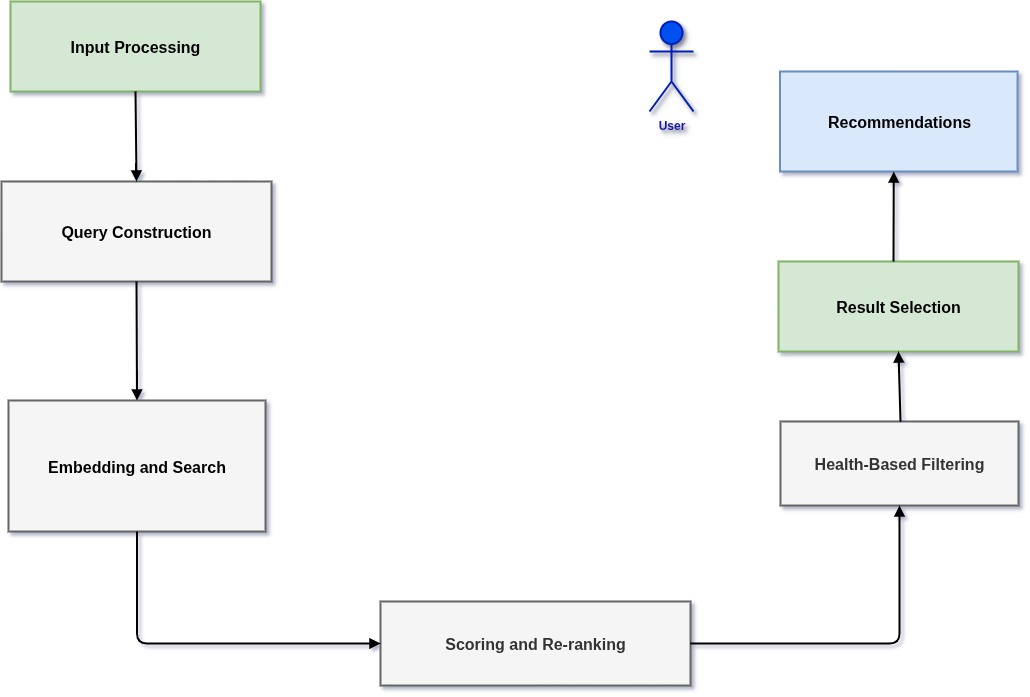
\includegraphics[width=0.9\textwidth]{images/CB_recommendation_workflow_simple.png}
\caption{Content-based recommendation workflow}
\label{fig:cb_workflow}
\end{figure}

\section{Collaborative Filtering Module}
\subsection{LightFM for Implicit Feedback}
LightFM implements matrix factorization optimized for implicit feedback (e.g., clicks, likes). It learns latent user and item embeddings to predict affinity.


\subsection{Interaction Matrix Design}
User actions are weighted to reflect preference strength:

\begin{table}[H]
\centering
\caption{Interaction types and weights}
\label{tab:interaction_weights}
\begin{tabular}{lcc}
\toprule
\textbf{Interaction} & \textbf{Weight} & \textbf{Interpretation} \\
\midrule
Liked & 1.0 & Strong positive \\
Visited & 0.5 & Mild interest \\
Disliked & -1.0 & Explicit negative \\
\bottomrule
\end{tabular}
\end{table}

\subsection{Loss Function Selection}
LightFM supports multiple loss functions:
\item \textbf{WARP}: Ignores negative feedback—unsuitable for our use case.
    \item \textbf{Logistic}: Requires explicit ratings—not applicable.
    \item \textbf{BPR (Bayesian Personalized Ranking)}: Optimizes pairwise ranking of liked vs. disliked/visited items.

We selected **BPR** to fully leverage explicit dislikes and ensure robust ranking.

\begin{figure}[H]
\centering
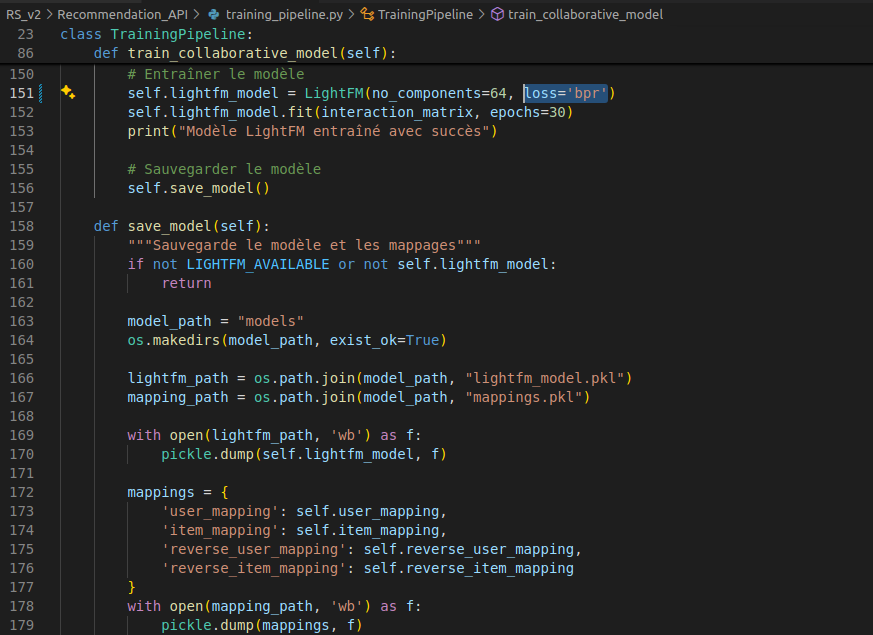
\includegraphics[scale=0.39]{images/loss_function_lightFM.png}
\caption{Training LightFM with BPR loss}
\label{fig:BPR_loss_function}
\end{figure}

\section{Scalability: Exact vs. Approximate Search}
\subsection{The Need for ANN in Production}
Exact cosine similarity search becomes infeasible beyond ~10K vectors. To ensure scalability, we benchmarked ChromaDB’s **HNSW-based ANN** against its default exact search.

\subsection{Theoretical Trade-offs}
\begin{table}[H]
\centering
\caption{Exact vs. HNSW search: key differences}
\label{tab:theoretical-comparison}
\resizebox{0.9\textwidth}{!}{%
\begin{tabular}{|l|c|c|}
\hline
\textbf{Feature} & \textbf{Exact Search} & \textbf{HNSW (ANN)} \\
\hline
Accuracy & 100\% & High (configurable) \\
Speed & Slow (O(n)) & Fast (sub-linear) \\
Memory & Low & Higher (graph index) \\
Scalability & <10K vectors & Millions of vectors \\
\hline
\end{tabular}
}
\end{table}

\subsection{Empirical Benchmark}
Tested on 23,000 products with 20,000 queries:

\begin{table}[H]
\centering
\caption{Performance benchmark}
\label{tab:benchmark-results}
\resizebox{0.7\textwidth}{!}{%
\begin{tabular}{|l|c|c|c|}
\hline
\textbf{Mode} & \textbf{Avg. Latency (ms)} & \textbf{Results/Query} & \textbf{Success Rate} \\
\hline
Exact & 187.4 & 10 & 100\% \\
HNSW & 178.08 & 10 & 100\% \\
\hline
\end{tabular}
}
\end{table}

HNSW delivers **5\% faster response times** with identical result quality at this scale—and will scale far better as the catalog grows. It is now the production default.

\section{Deployment and Integration}
\subsection{FastAPI Backend}
The system is exposed via a private FastAPI service with a single endpoint:
\begin{verbatim}
POST /recommend
\end{verbatim}
Input: \texttt{user\_id}, \texttt{ean} (optional), \texttt{limit}, \texttt{recommendation\_type}.

\begin{figure}[H]
\centering
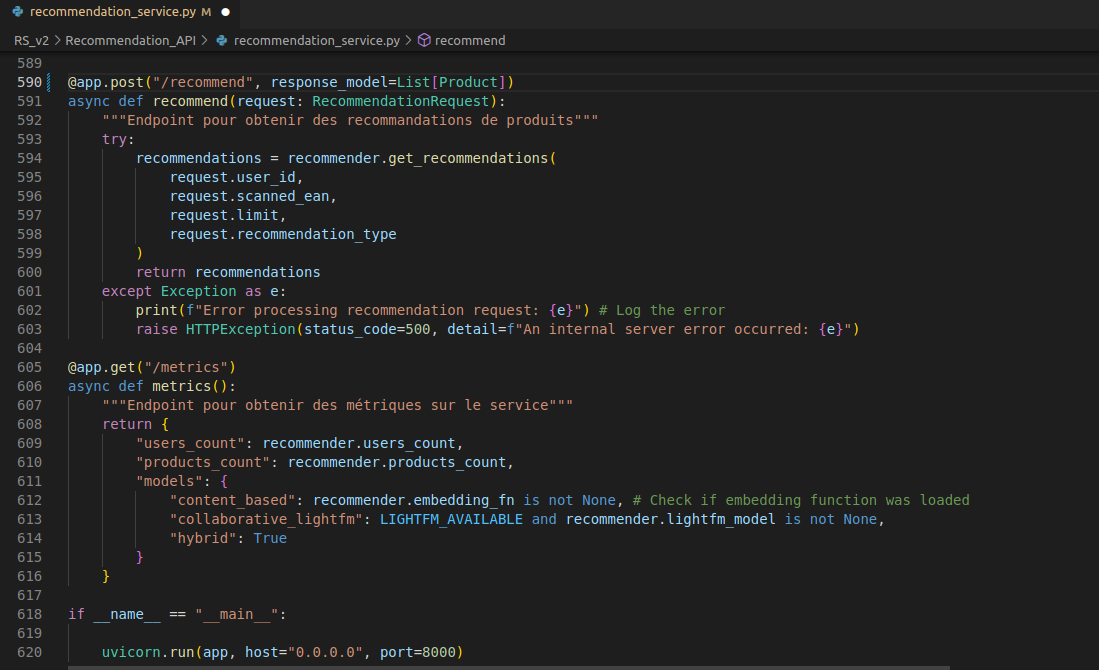
\includegraphics[scale=0.35]{images/deploy_RS.png}
\caption{Deployment architecture with FastAPI}
\label{fig:Deploy_RS}
\end{figure}

\subsection{Multi-Modal Recommendation Modes}
The \texttt{recommendation\_type} parameter supports:
\begin{enumerate}
    \item \texttt{"collaborative"} – LightFM only
    \item \texttt{"content"} – ChromaDB only
    \item \texttt{"hybrid"} – Weighted fusion (60/40)
\end{enumerate}

Internal access only (mobile app + dev team), with full documentation via Swagger UI.


\section*{Conclusion}
This chapter has outlined the architectural and algorithmic foundations
of the VitamiNurse recommendation system. The system employs a
modular, hybrid architecture that separates collaborative and contentbased filtering to achieve a balance between scalability and precision.
Integration of ChromaDB with HNSW indexing facilitates efficient semantic analysis of user needs and product attributes. Additionally, the
LightFM model, trained using a Bayesian Personalized Ranking (BPR)
loss function, effectively captures dynamic user preferences derived from
implicit feedback.
By concentrating on the user health condition, allergies and health goals,
the recommendation system suggests more healthy and personalized
products. However, providing effective guidance also requires an intuitive
and interactive tool. To address this need, the next chapter introduces
VitamiNurse AI assistant, designed to deliver real-time, conversational
support that bridges large language models with user-friendly interaction.